\documentclass[12pt,prb,aps,epsf]{article}
\usepackage[utf8]{inputenc}
\usepackage{amsmath}
\usepackage{amsfonts}
\usepackage{amssymb}
\usepackage{graphicx} 
\usepackage{latexsym} 
\usepackage[toc,page]{appendix}
\usepackage{listings}
\usepackage{xcolor}
\usepackage{soul}
\usepackage[T1]{fontenc}
\usepackage{amsthm}
\usepackage{mathtools}
\usepackage{setspace}
\usepackage{array,multirow,makecell}
\usepackage{geometry}
\usepackage{textcomp}
\usepackage{float}
%\usepackage{siunitx}
\usepackage{cancel}
%\usepackage{tikz}
%\usetikzlibrary{calc, shapes, backgrounds, arrows, decorations.pathmorphing, positioning, fit, petri, tikzmark}
\usepackage{here}
\usepackage{titlesec}
%\usepackage{bm}
\usepackage{bbold}
\geometry{hmargin=2cm,vmargin=2cm}

\begin{document}
	
	\title{MP 15 Production et mesures de champs magnétiques}
		\author{Naïmo Davier}
		\date{Agrégation 2019}
		
	\maketitle
	
	\tableofcontents
	
	\pagebreak
	
\subsection{Introduction}
On va mesurer des champs de différents entre de grandeur en amplitude.
	
\section{Mesure du champ magnétique terrestre $B_H$}
\textbf{Montage de physique} de \textit{J.P Bellier} p52.\\

\begin{figure}[h]
 	\centering 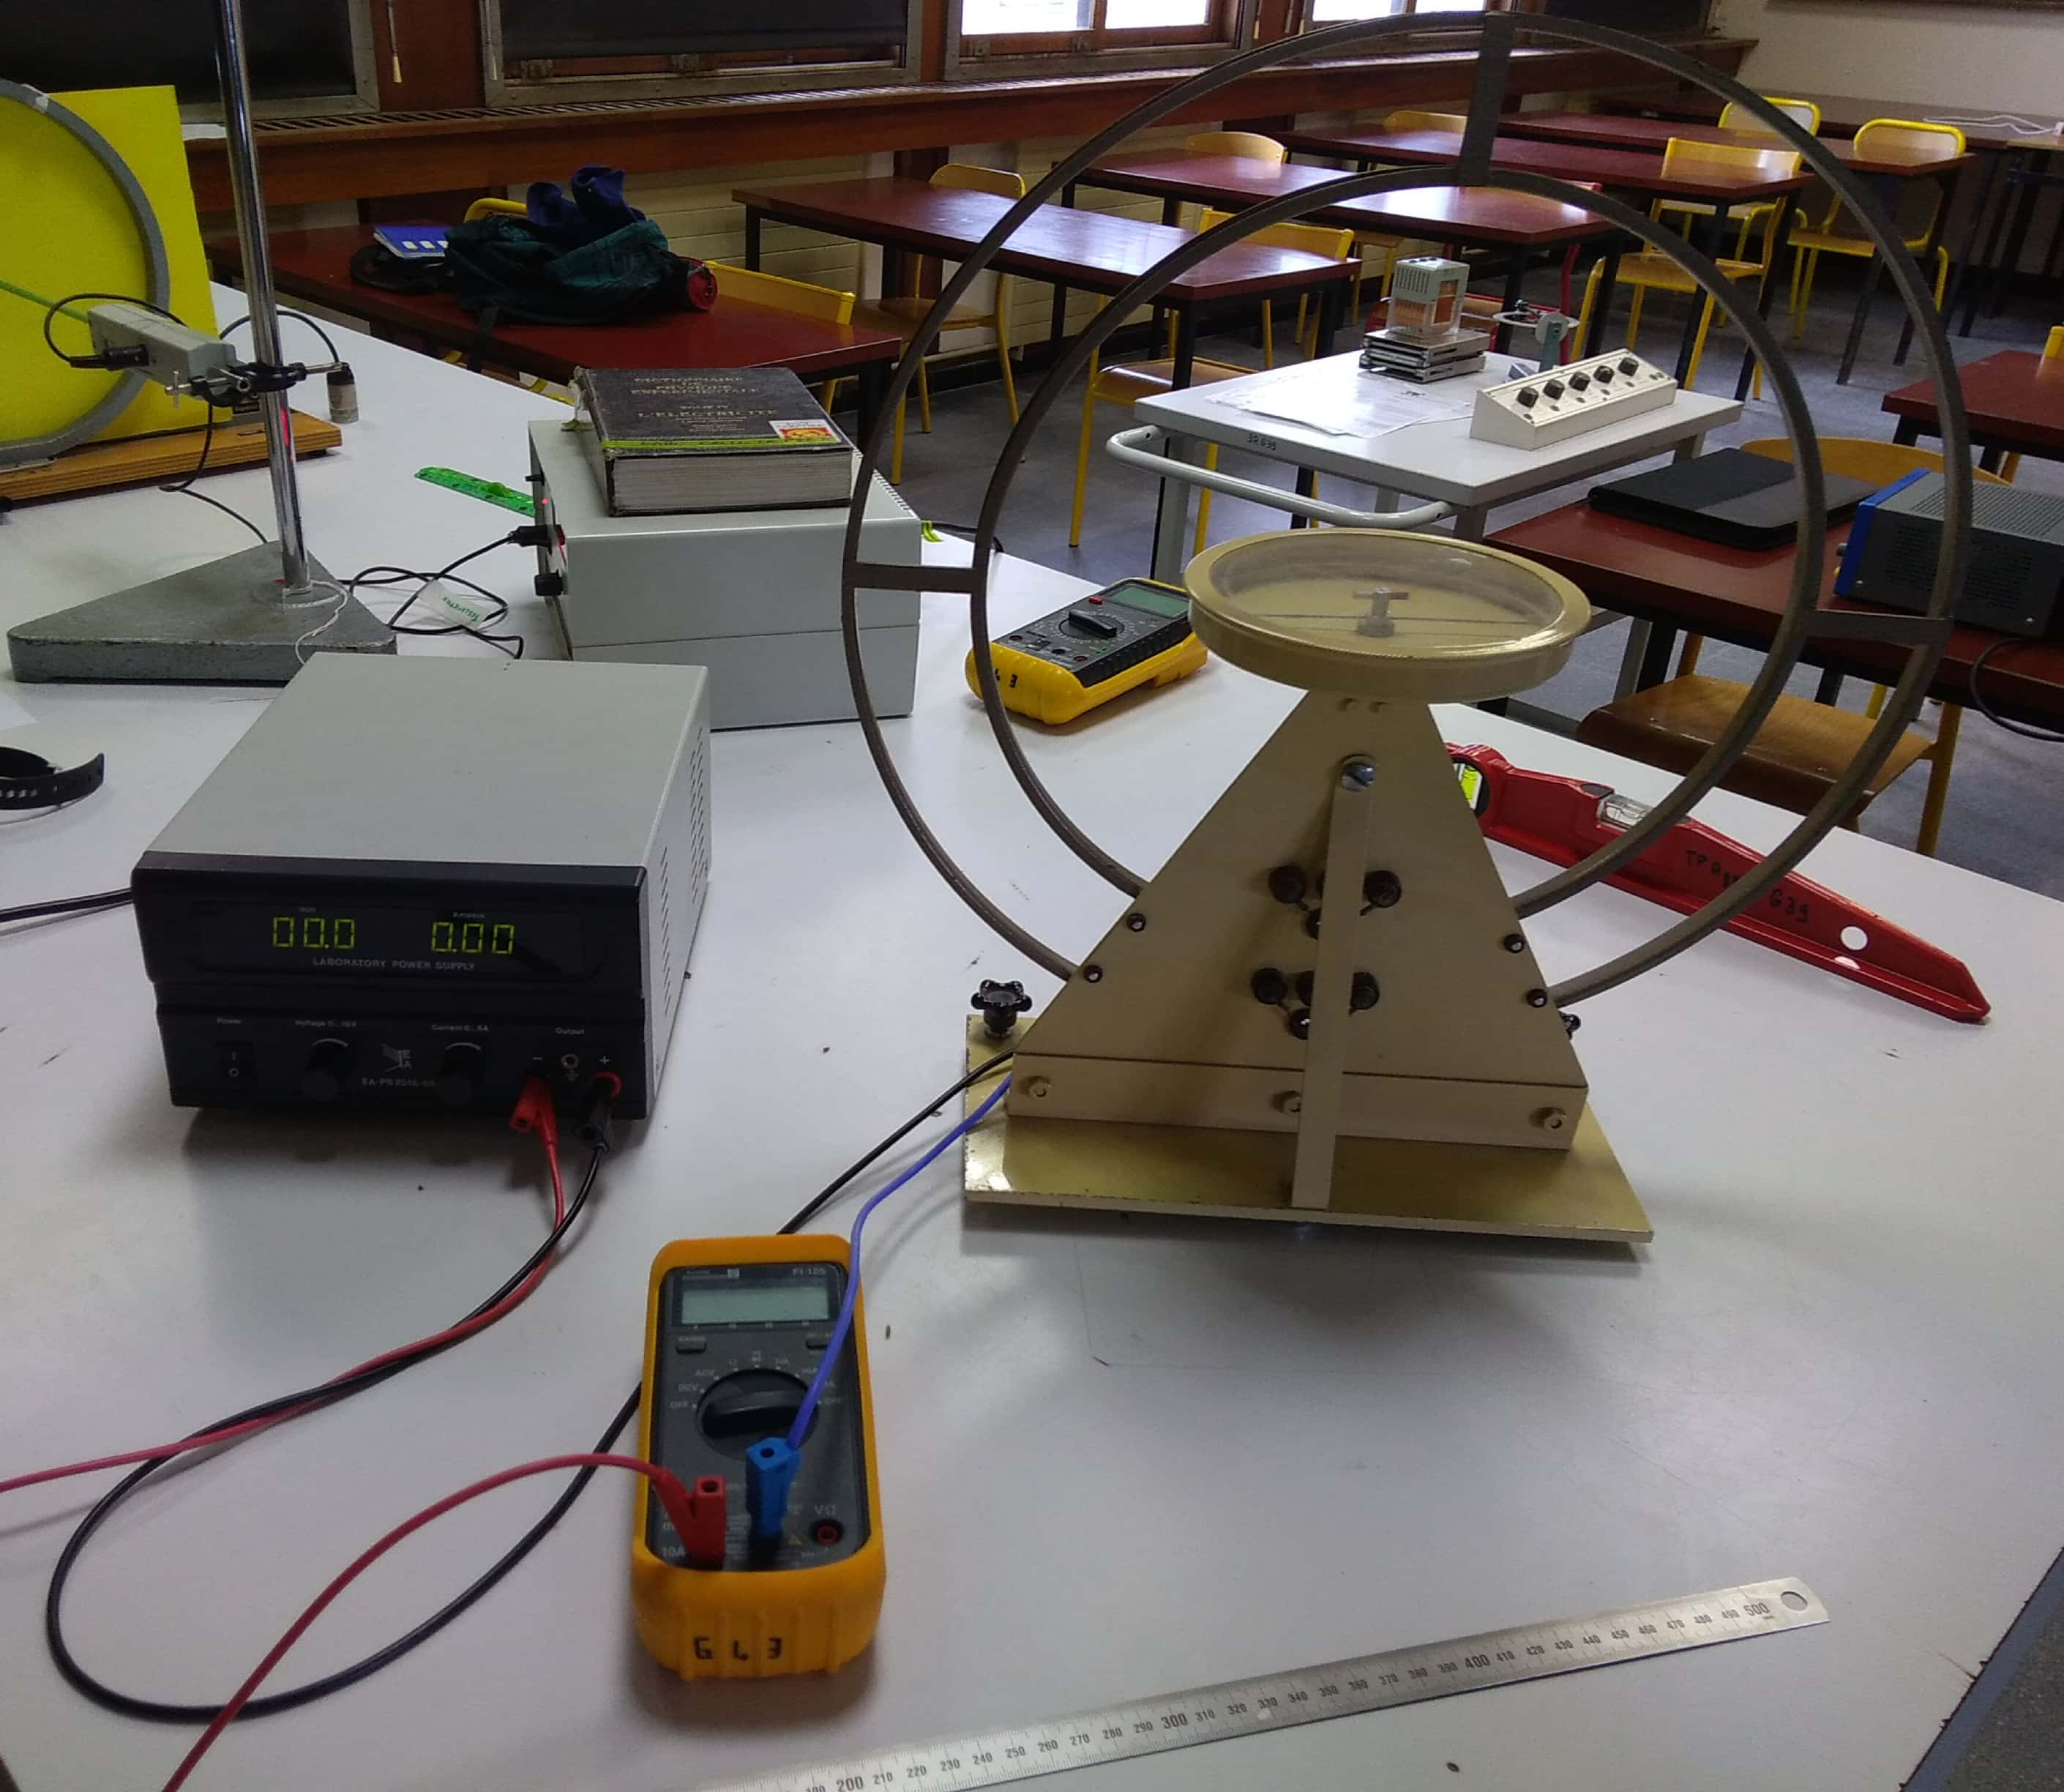
\includegraphics[width=8cm]{chp_terrestre}
\end{figure}
On veut effectuer une mesure de la composante horizontale du champ magnétique terrestre. Pour cela on dispose d'une boussole de précision placée au centre d'une bobine de grand diamètre ($D\simeq30$ cm). On relie cette bobine à un générateur courant tension, tout en plaçant un ampèremètre pour contrôler le courant $I$ avec précision.\\
La bobine génère en son centre un champ magnétique 
\begin{eqnarray}
\vec{B}_0 = \frac{\mu_0NI}{2R}\vec{e}_n
\end{eqnarray}
avec $R = 15,2\pm0,1$ cm le rayon de la bobine, $N = 10$ le nombre de spires, et $\vec{e}_n$ le vecteur normal au plan de la bobine (choisi avec la règle de la main droite).\\

On en déduit qu'au centre de la bobine, la boussole voit un champ 
\begin{eqnarray}
\vec{B} = \vec{B}_0 + \vec{B}_H
\end{eqnarray}
et va donc s'aligner selon ce champ. On place la bobine de telle sorte à avoir $\vec{B}_H\perp \vec{B}_0$ et  définit $\alpha$ l'angle entre $\vec{B}$ et $\vec{B}_H$, on a alors
\begin{eqnarray}
\tan(\alpha) = \frac{B_0}{B_H} = \frac{\mu_0NI}{2RB_H}
\end{eqnarray} 
On va donc tracer $\tan(\alpha) = f(I)$ et modéliser le résultat par une droite pour effectuer une mesure de $B_H$. Afin d'être plus précis on mesure l'angle pour I et -I et on prend la moyenne des deux angles mesurés, on s'affranchit alors du choix de l'origine des angles. On a s'attend à avoir $B_H \simeq 2.10^{-5}$ T et on mesure ici $B_H =2,18\pm0,06\, .10^{-5}$ T, on a donc un accord à $3\sigma$ entre la valeur attendue (tabulé) et celle mesurée, la manip semble donc pertinente.

\section{Production d'un champ magnétique par une spire plate}
\textbf{Montage de physique} de \textit{J.P Bellier} p51.\\

\begin{figure}[h]
	\centering 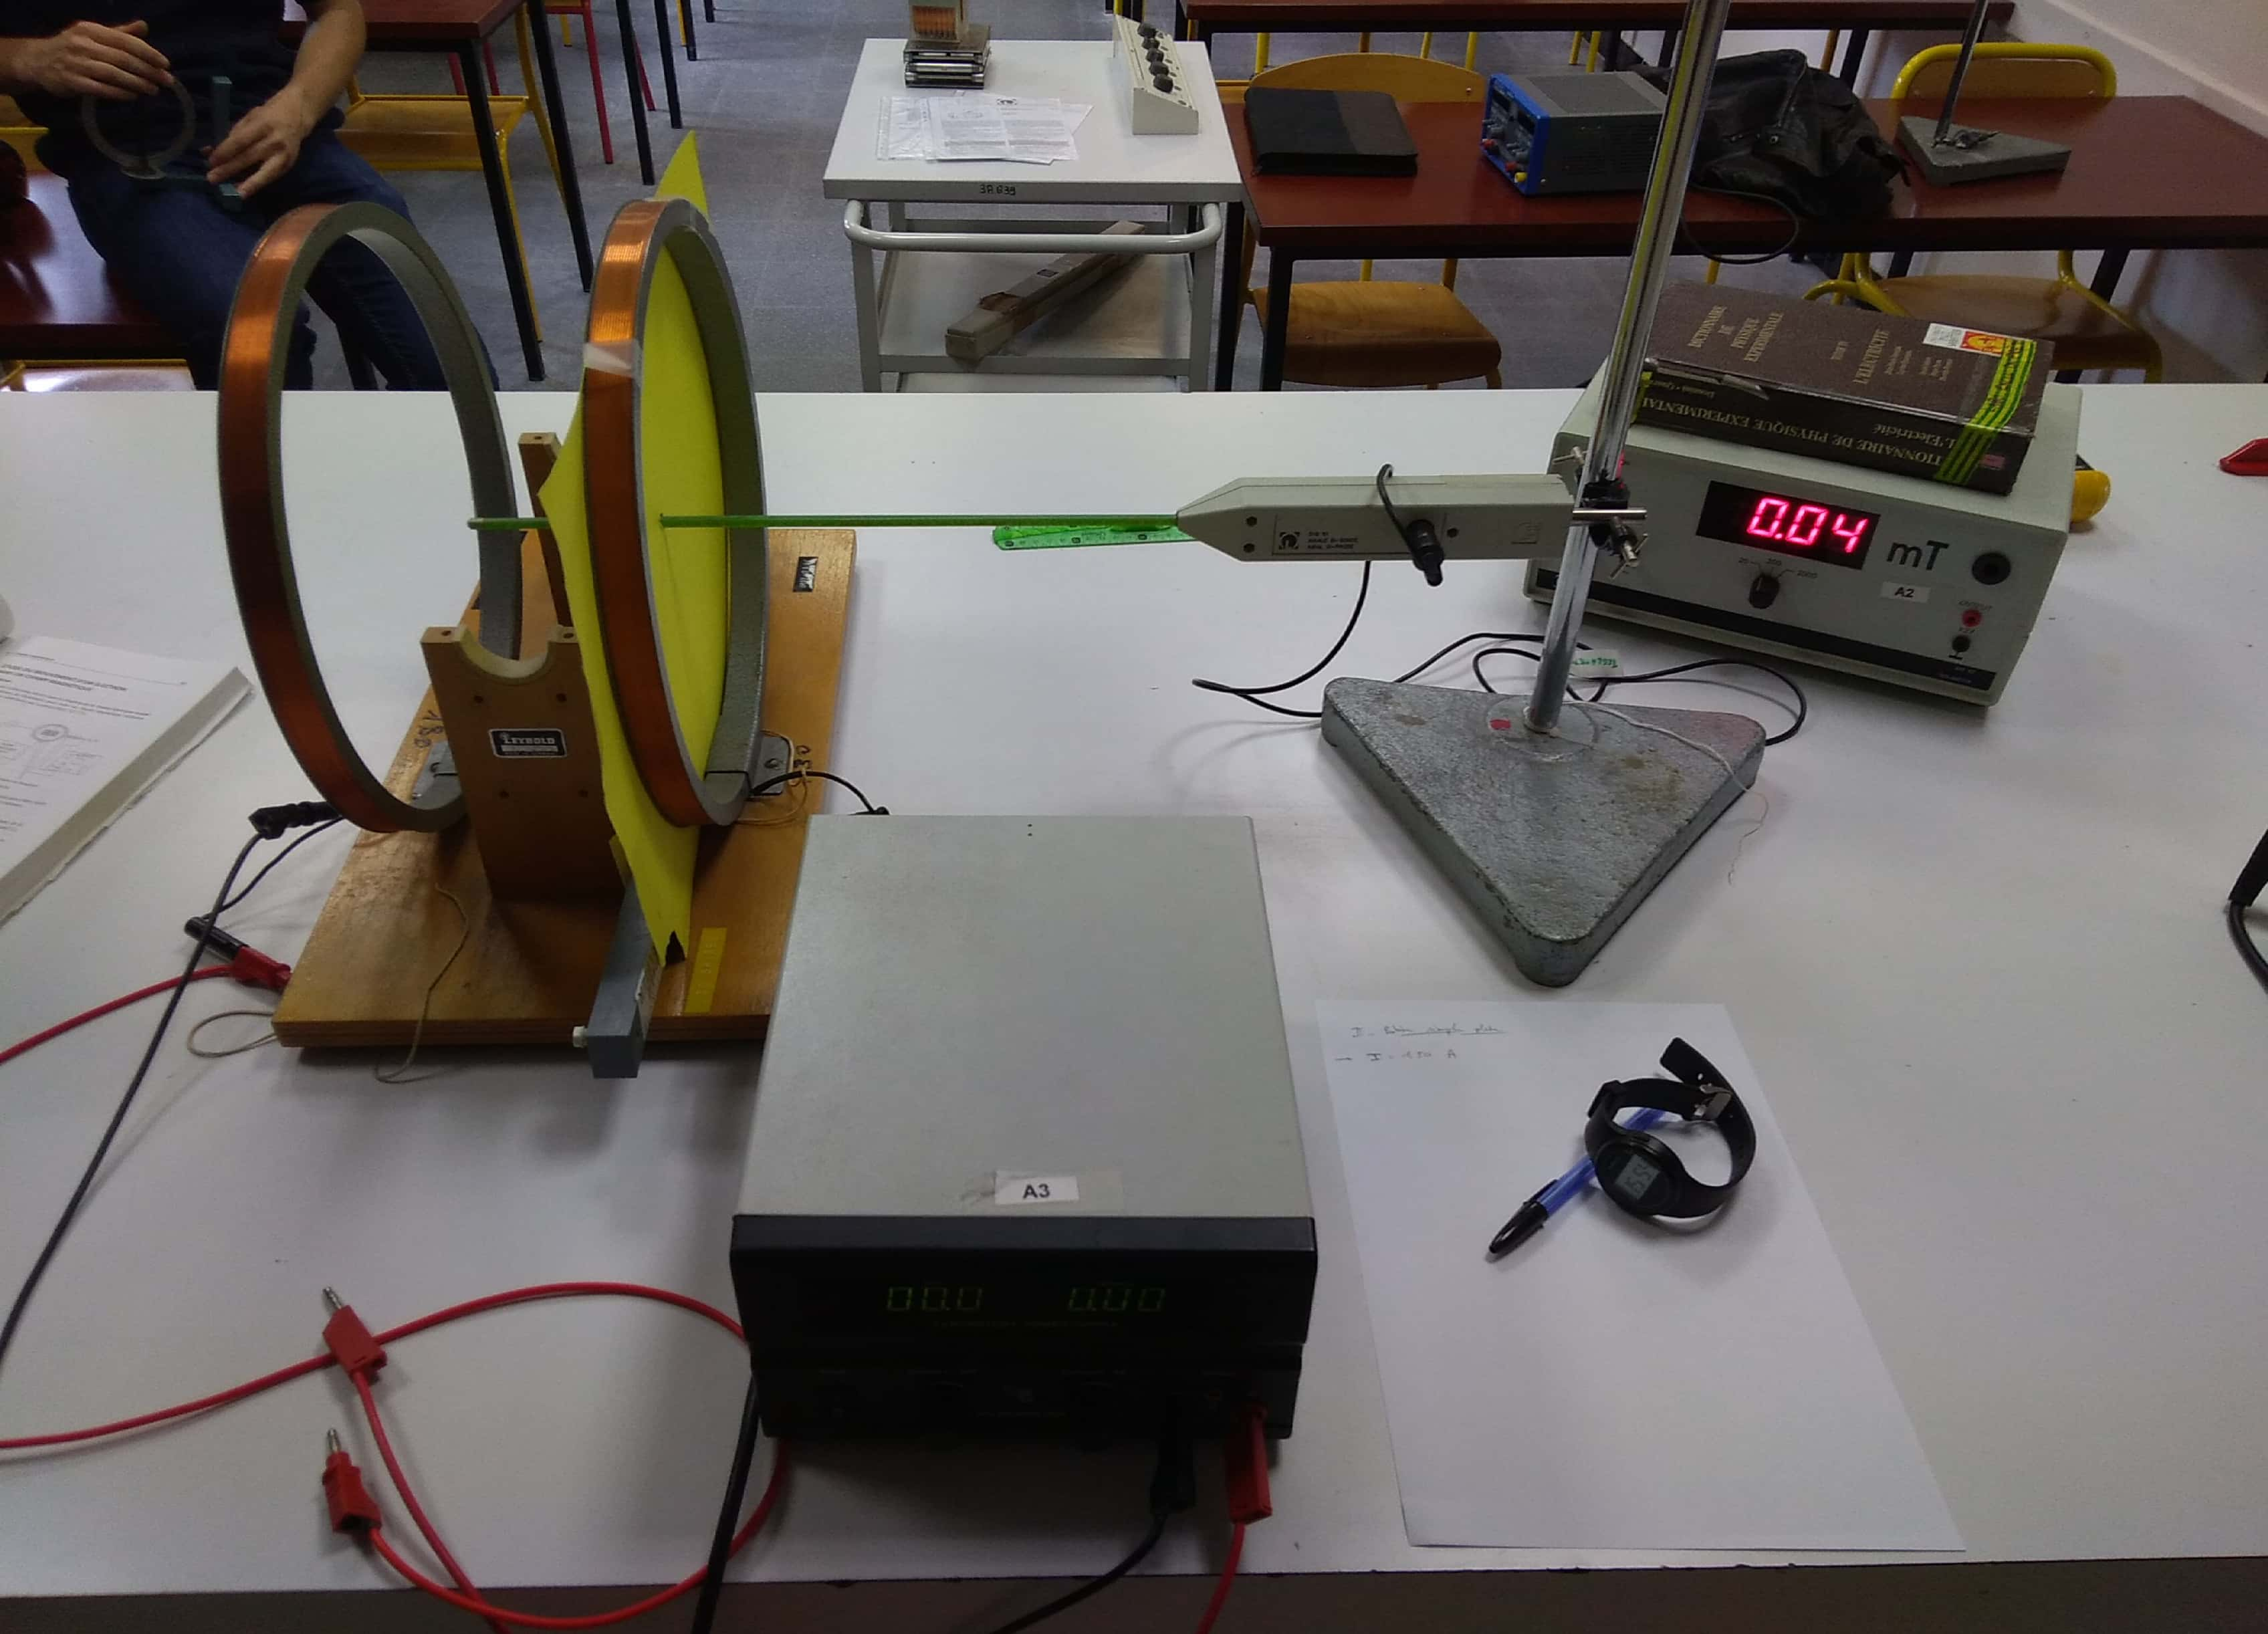
\includegraphics[width=10cm]{bobine_plate}
\end{figure}

On regarde ici une spire plate (1 cm d'épaisseur environ) et de grand diamètre (environ 30cm). On va ici établir le profil du champ axial sur l'axe central de la bobine, pour ça on utilise une sonde à effet Hall longitudinale que l'on avance petit à petit sur l'axe, tout en relevant sa position pour chaque point (on a pour cela formé un plan horizontal à l'aide d'une feuille, servant d'origine pour la mesure de longueur).\\
On obtient alors un profil de champ $B(x)$ que l'on peut tracer sur régressi, on observe alors une courbe en cloche que l'on peut modéliser par l'expression 
\begin{eqnarray}
B(x) = \frac{\mu_0 NI}{2R} \left(1+\left(\frac{x-x_0}{R}\right)^2\right)^{-3/2}
\end{eqnarray}
avec $x_0$ la position de du centre de la bobine. La modélisation par cette fonction nous permet alors de comparer les coefficients obtenus avec les coefficients du modèle (basé sur Biot-Savart).

\section{Production d'un champ magnétique par un électroaimant}
\textit{Quaranta} \textbf{Tome IV l'électricité} p149.\\

\begin{figure}[h]
	\centering 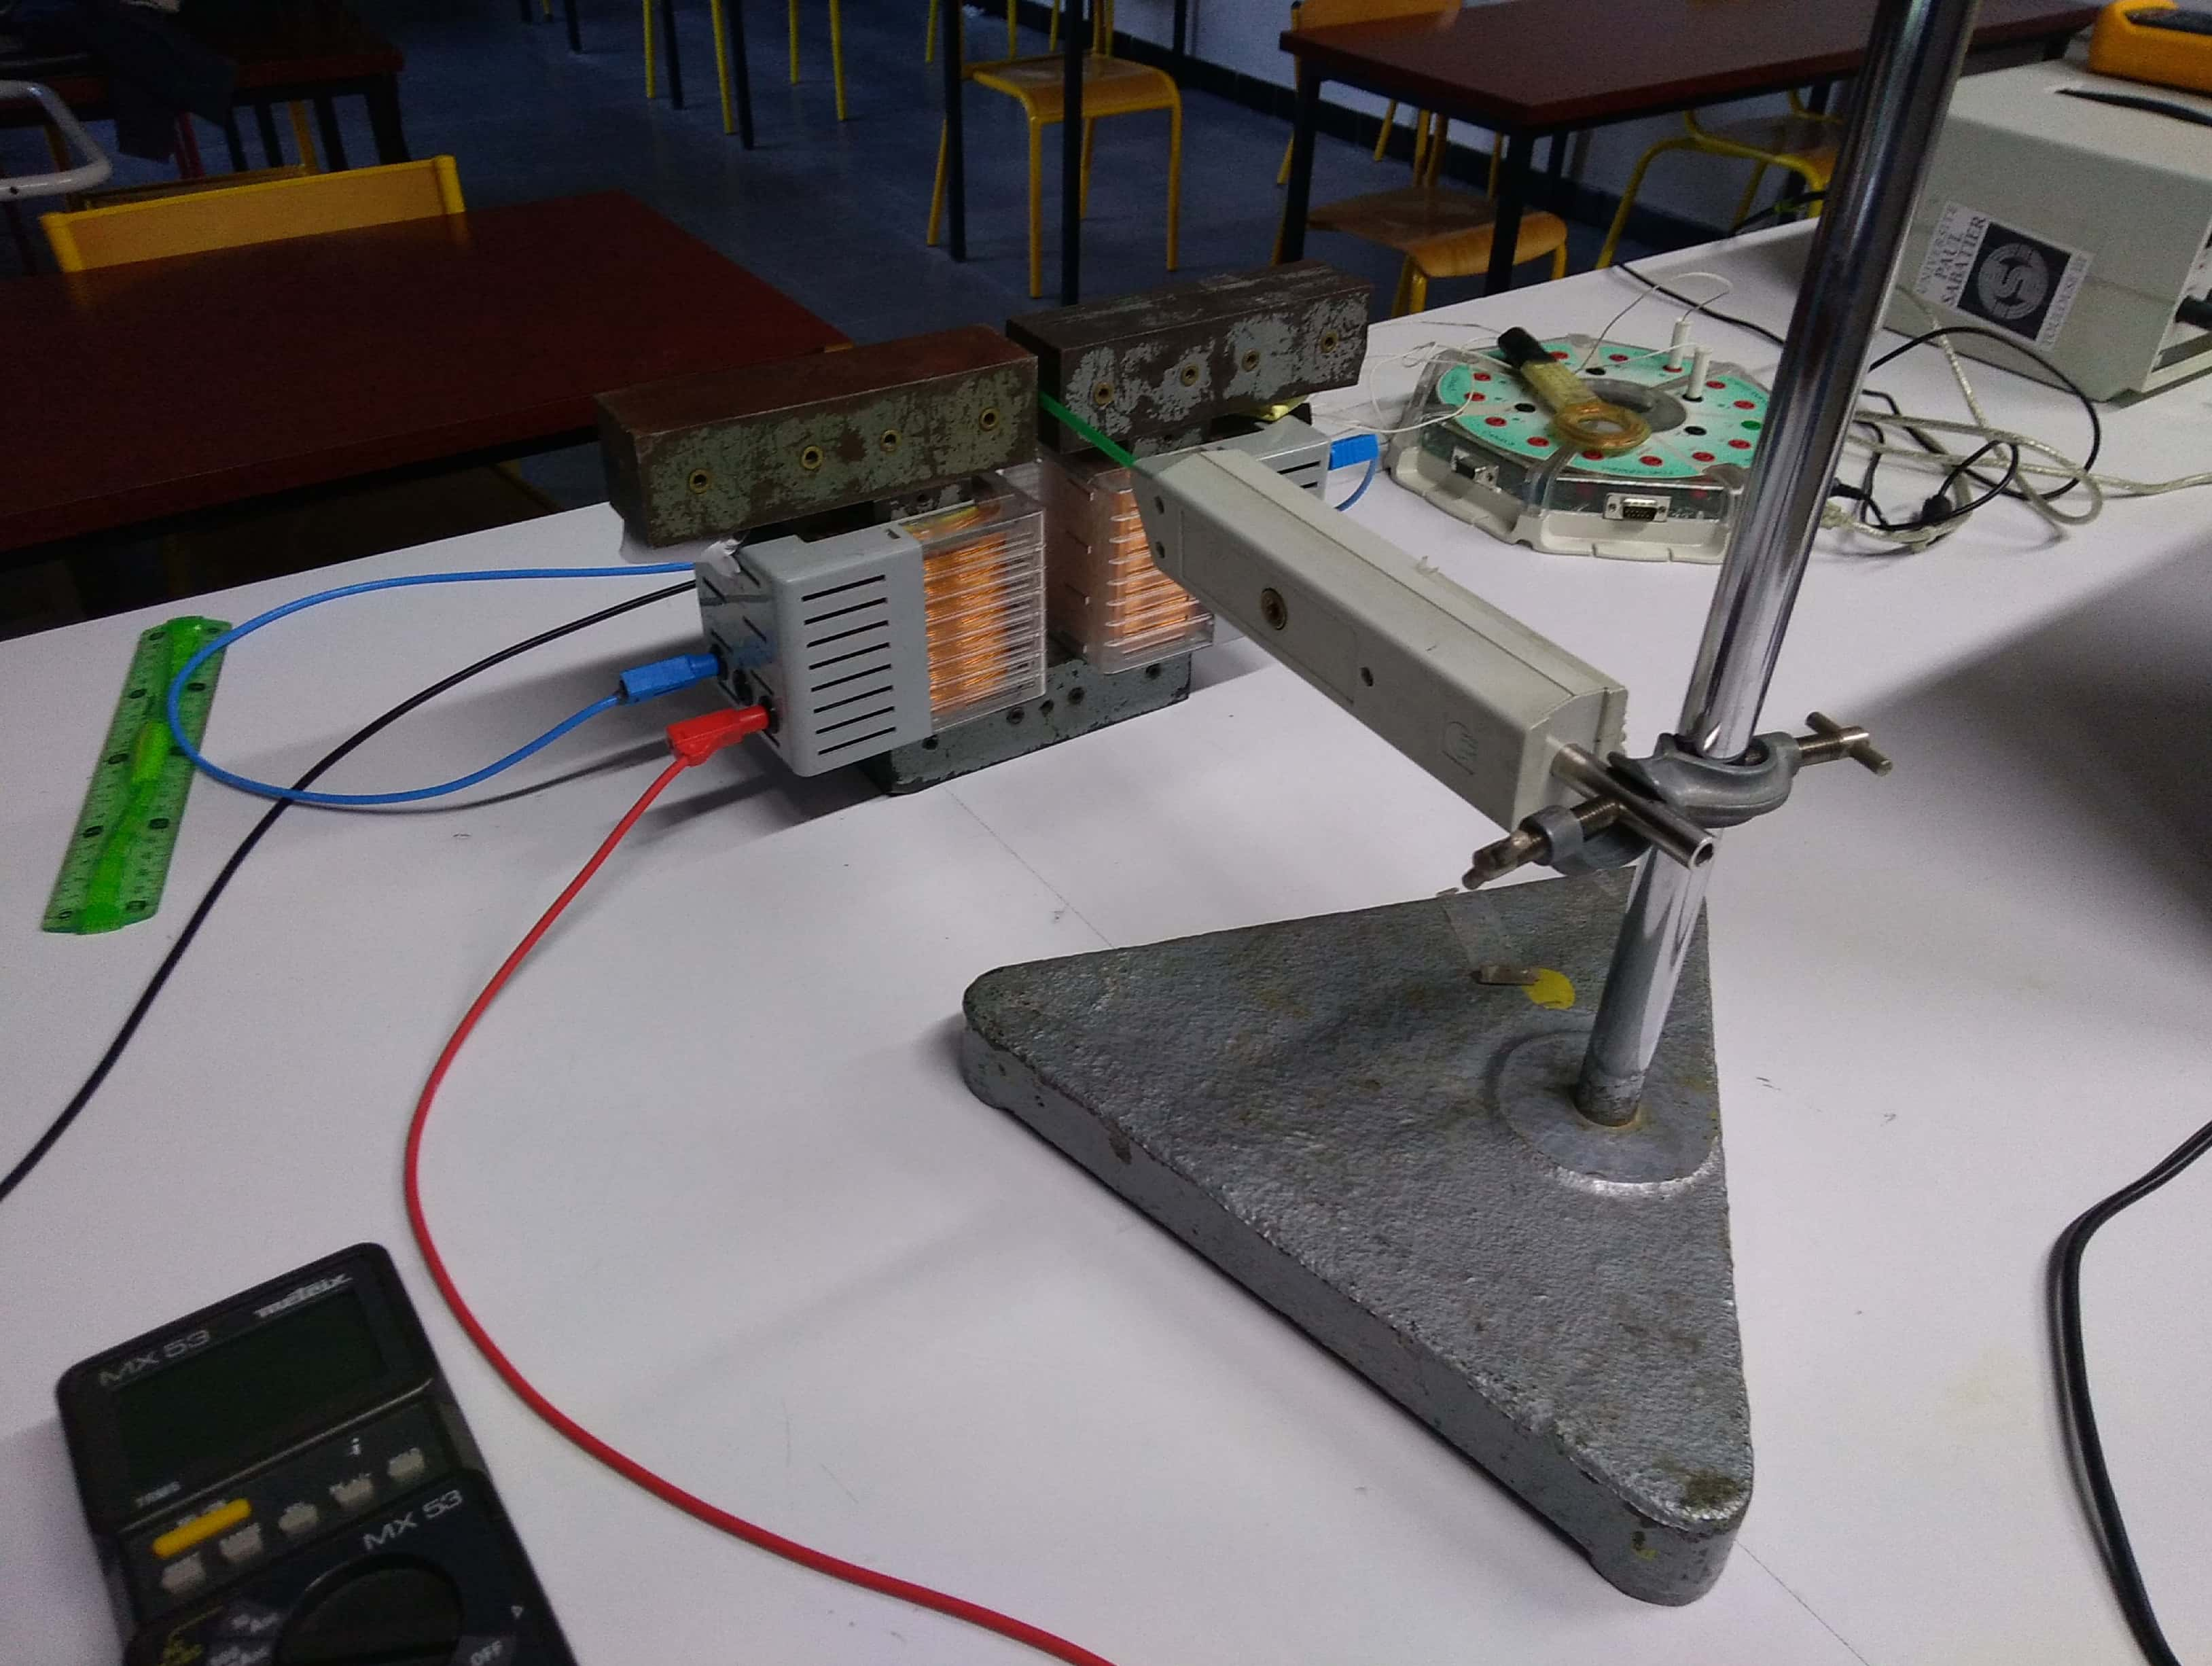
\includegraphics[width=10cm]{entrefer}
\end{figure}
On forme un entrefer à l'aide d'un U et de deux lingots en ferromagnétique dur qui est feuilleté. On place deux bobines sur le U de telle sorte à générer un champ magnétique tournant intense (de l'ordre de 500 mT).\\

On réalise une mesure du champ dans l'entrefer en fonction la largeur $e$ de l'entrefer, et on trace alors 
\begin{eqnarray}
B = f(1/e)
\end{eqnarray}
puisque l'on s'attend à avoir 
\begin{eqnarray}
B = \frac{\mu_0 NI}{e}
\end{eqnarray}
sous la condition $e \gg \frac{l}{\mu_r}$, avec $l$ la longueur moyenne de l'entrefer (ici $\simeq 45$ cm) et $\mu_r$ la perméabilité relative du matériau. On obtient une droite affine avec un très léger offset dû au fait que le teslamètre est imparfait et donne un léger offset même en faisant le 0.\\
On en déduit que l'intensité du champ magnétique produit est inversement proportionnelle à l'épaisseur de l'entrefer en réalisant une modélisation de la courbe obtenue, afin de confirmer notre modèle.

\section{Mesure de champ avec un fluxmètre}

\section{Conclusion}
On a vu différentes manières de générer des champs, notamment à l'aide de bobines. Pour obtenir des champs plus importants il faut s'intéresser aux camp pulsés qui peuvent atteindre quelques centaines de teslas. Ouverture aux champs variable, qui sont notamment utilisés dans les moteurs.

\section*{Questions}
Pour la première manip, y a t'il un moyen de mesurer le rayon de la spire autrement qu'à la règle ?\\
Oui on peut mesurer le champ au centre et appliquer la formule de la partie 2, en connaissant N et I.\\

D'où vient le champ magnétique terrestre ?\\

Pour la seconde manip, existe t-il une autre manipulation qui permettrait de déterminer le rayon de la spire ?\\
Ou on trace B(I) et on en déduit une mesure de R.\\

Que dit la documentation du teslamètre concernant les incertitudes liées au résultat affiché ?\\

Quels sont les facteurs d'élargissement ?\\

Quel est l'avantage de l'électroaimant ?\\
L'utilisation d'un ferromagnétique amplifie le champ produit par les bobines, de plus la géométrie de l'entrefer assure un champ magnétique uniforme, ce dernier étant guidé par la ferromagnétique. De plus ce champ est d'autant plus intense que $e$ est faible : permet d'influer sur le champ via la géométrie du système.\\

Pourquoi ne pas avoir pris des éléments ferro tronconiques ?\\

Etes vous sur que l'on doive aller vers des champs pulsés pour avoir des champ de plus de 1T ?\\
On peut tout d'abord améliorer notre électroaimant pour atteindre des champ de quelques teslas. On peut aussi utiliser des bobines faites à l'aide de supraconducteurs pour obtenir de grands courants et ainsi de grands champs, on est tout de même limité par la transition supra-normal à trop fort champ.

\section*{Remarques}
Pour mesurer le rayon des spires il est plus précis, surtout pour la deuxième, de mesurer le rayon en traçant B(I).\\
Il y a mesure dans le titre, donc placer la plaquette à effet Hall à la place de la mesure du champ terrestre peut être pertinent.\\
Si on ne fait pas la plaquette à effet Hall alors il ne faut pas perdre de temps à en expliquer le principe, l'attendre aux questions.








\end{document}